% Fig. 1. (a) The task on an invented post. (b) How one generated training row is made.
% (c) The five training conditions for one held-out fold. The post was written for illustration and is not
% from the dataset. Built by figures.py (pdflatex, SOURCE_DATE_EPOCH=0). Drawn at print size for
% \textwidth (181 mm). Colors carry the logic: blue real, orange generated, green evidence, purple labels.
\documentclass[border=1pt]{standalone}
\usepackage[T1]{fontenc}
\usepackage{newtxtext}
\usepackage{tikz}
\usetikzlibrary{arrows.meta}
\pdfinfoomitdate=1
\pdftrailerid{}
\pdfsuppressptexinfo=-1

% Fills: draw.io default hues one step lighter; outlines at the defaults (NRCP schematic style).
\definecolor{realFill}{HTML}{A9D0FF}  \definecolor{realLine}{HTML}{6C8EBF}
\definecolor{dupFill}{HTML}{DCEBFF}
\definecolor{genFill}{HTML}{F5C38D}   \definecolor{genLine}{HTML}{D79B00}
\definecolor{outFill}{HTML}{AADEA9}   \definecolor{outLine}{HTML}{82B366}
\definecolor{labFill}{HTML}{E1D5E7}   \definecolor{labLine}{HTML}{9673A6}

\newcommand{\body}{\fontsize{8}{9.6}\selectfont}
\newcommand{\note}{\fontsize{7}{8.4}\selectfont}
\newcommand{\panel}[2]{{\fontsize{9}{10.8}\selectfont\bfseries #1}\ {\body #2}}
\newcommand{\hlq}[1]{{\setlength{\fboxsep}{0.8pt}\kern-\fboxsep\colorbox{outFill}{#1}\kern-\fboxsep}}
% Chips, 5 mm tall like the ladder cells; colorboxes, not nested tikz nodes, so they inherit no node options.
\newcommand{\chip}[1]{{\setlength{\fboxsep}{2.3pt}\colorbox{labFill}{\strut#1}}}
\newcommand{\evid}[1]{{\setlength{\fboxsep}{2.3pt}\colorbox{outFill}{\strut#1}}}

% Grid (mm): columns (a) 0-52, (b) 62-116, (c) 126-181; titles at y = 0, content from y = -6 to -60.
\tikzset{
  every picture/.style={line width=0.5pt, x=1mm, y=1mm},
  title/.style={anchor=north west, inner sep=0pt},
  head/.style={anchor=north west, inner sep=0pt, font=\body\bfseries},
  item/.style={anchor=north west, inner sep=0pt, font=\body},
  cell/.style={draw=labLine, minimum width=13mm, minimum height=5mm, inner sep=0pt, font=\body, anchor=north west},
  wide/.style={minimum width=54mm, inner xsep=0pt, font=\body, align=center},
  post/.style={draw=realLine, fill=realFill, minimum width=9mm, minimum height=8mm, inner sep=0pt},
  bar/.style={draw, minimum height=5mm, minimum width=13mm, inner sep=0pt, font=\note, anchor=west},
  flow/.style={-{Latex[length=4pt, width=3.5pt]}, line width=0.6pt, draw=black!80},
  ctx/.style={-{Latex[length=3pt, width=2.5pt]}, dashed, draw=realLine},
}

\begin{document}
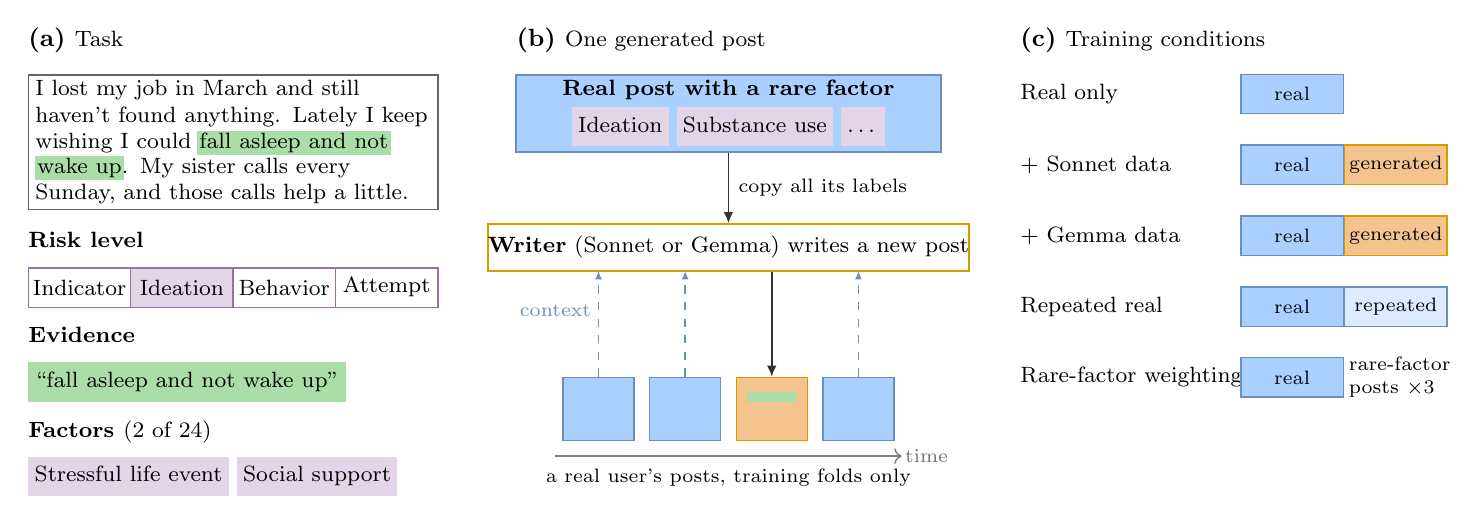
\begin{tikzpicture}
  % ---------------- (a) the task: one post, three outputs
  \node[title] at (0, 0) {\panel{(a)}{Task}};
  \node[draw=black!60, anchor=north west, inner xsep=2.5pt, inner ysep=2pt, font=\body, align=left,
        text width=52mm-5pt] at (0, -6)
    {I lost my job in March and still\\
     haven't found anything. Lately I keep\\
     wishing I could \hlq{fall asleep and not}\\
     \hlq{wake up}. My sister calls every\\
     Sunday, and those calls help a little.};
  \node[head] at (0, -26) {Risk level};
  \foreach \l/\c [count=\i from 0] in {Indicator/white, Ideation/labFill, Behavior/white, Attempt/white}
    \node[cell, fill=\c] at (\i*13, -30.5) {\l};
  \node[head] at (0, -38) {Evidence};
  \node[item] at (0, -42.5) {\evid{``fall asleep and not wake up''}};
  \node[head] at (0, -50) {Factors \textmd{(2 of 24)}};
  \node[item] at (0, -54.5) {\chip{Stressful life event}\ \chip{Social support}};

  % ---------------- (b) one generated post, centred on x = 89
  \node[title] at (62, 0) {\panel{(b)}{One generated post}};
  \node[wide, draw=realLine, fill=realFill, anchor=north, inner ysep=2pt] (carrier) at (89, -6)
    {\textbf{Real post with a rare factor}\\[1.5pt]\chip{Ideation}\ \chip{Substance use}\ \chip{\dots}};
  \node[wide, draw=genLine, fill=white, minimum height=6mm] (writer) at (89, -28) {\textbf{Writer} (Sonnet or Gemma) writes a new post};
  \draw[flow] (carrier) -- node[right, font=\note] {copy all its labels} (writer);
  \foreach \x in {72.5, 83.5, 105.5} {
    \node[post] (p) at (\x, -48.5) {};
    \draw[ctx] (p.north) -- (\x, -31);
  }
  \node[font=\note, text=realLine, anchor=east, inner sep=1pt] at (72, -36) {context};
  \node[post, draw=genLine, fill=genFill] (gen) at (94.5, -48.5) {};
  \fill[outFill] ([xshift=1.5mm, yshift=-2mm]gen.north west) rectangle ([xshift=-1.5mm, yshift=-3.2mm]gen.north east);
  \draw[flow] (gen.north |- writer.south) -- (gen);
  \draw[->, draw=black!50] (67, -54.5) -- (111, -54.5) node[right, inner sep=1pt, font=\note, text=black!55] {time};
  \node[font=\note, anchor=north, inner sep=0pt] at (89, -56) {a real user's posts, training folds only};

  % ---------------- (c) five conditions, one budget
  \node[title] at (126, 0) {\panel{(c)}{Training conditions}};
  \foreach \y/\name/\extra/\fc/\lc in {
      -8.5/Real only///,
      -17.5/+ Sonnet data/generated/genFill/genLine,
      -26.5/+ Gemma data/generated/genFill/genLine,
      -35.5/Repeated real/repeated/dupFill/realLine} {
    \node[font=\body, anchor=west, inner sep=0pt] at (126, \y) {\name};
    \node[bar, fill=realFill, draw=realLine] (r) at (154, \y) {real};
    \if\relax\fc\relax\else\node[bar, fill=\fc, draw=\lc] at (r.east) {\extra};\fi
  }
  \node[font=\body, anchor=west, inner sep=0pt] at (126, -44.5) {Rare-factor weighting};
  \node[bar, fill=realFill, draw=realLine] (r) at (154, -44.5) {real};
  \node[font=\note, anchor=west, align=left, inner xsep=1.5pt] at (r.east) {rare-factor\\posts $\times$3};
\end{tikzpicture}
\end{document}
